% This is samplepaper.tex, a sample chapter demonstrating the
% LLNCS macro package for Springer Computer Science proceedings;
% Version 2.20 of 2017/10/04
%
\documentclass[runningheads]{llncs}
%
\usepackage{graphicx}
\usepackage{color}
\usepackage{amsmath}
\usepackage{amssymb}
\usepackage{bcprules, proof}
\usepackage{fancybox}
\usepackage{mathtools}
\usepackage{float}
\usepackage{xparse}
% \usepackage{ebproof}
\usepackage{lscape}
\usepackage{mdframed}

% Used for displaying a sample figure. If possible, figure files should
% be included in EPS format.
%
% If you use the hyperref package, please uncomment the following line
% to display URLs in blue roman font according to Springer's eBook style:
% \renewcommand\UrlFont{\color{blue}\rmfamily}

\newcommand{\red}[1]{\textcolor{red}{#1 }}
\newcommand{\blue}[1]{\textcolor{blue}{#1 }}

\newcommand{\LTP}{$\lambda^{\triangleright\%}$\ }
\newcommand{\LMD}{$\lambda^{\textrm{MD}}$\ }
\newcommand{\LLF}{$\lambda^{\textrm{LF}}$\ }

\newcommand{\G}{\Gamma}
\newcommand{\D}{\Delta}
\newcommand{\V}{\vdash_\Sigma}
\newcommand{\VT}{\vdash\hspace{-.50em}\raisebox{0.28em}{\tiny{$\TB$}}}
\newcommand{\iskind}{\text{\ kind}}
\newcommand{\TW}{\triangleright}
\newcommand{\TWL}{\triangleleft}
\newcommand{\F}{\forall}
\newcommand{\TB}{\blacktriangleright}
\newcommand{\TBL}{\blacktriangleleft}
\newcommand{\E}{\equiv}
\newcommand{\FV}{\text{FV}}
\newcommand{\FTV}{\text{FSV}}

\newcommand{\WStar}{\textsc{W-Star}}
\newcommand{\WAbs}{\textsc{W-Abs}}
\newcommand{\WCsp}{\textsc{W-Csp}}
\newcommand{\WApp}{\textsc{W-App}}
\newcommand{\WTW}{\textsc{W-$\TW$}}

\newcommand{\KVar}{\textsc{K-Var}}
\newcommand{\KAbs}{\textsc{K-Abs}}
\newcommand{\KApp}{\textsc{K-App}}
\newcommand{\KConv}{\textsc{K-Conv}}
\newcommand{\KTW}{\textsc{K-$\TW$}}
\newcommand{\KTWL}{\textsc{K-$\TWL$}}
\newcommand{\KGen}{\textsc{K-Gen}}
\newcommand{\KCsp}{\textsc{K-Csp}}

\newcommand{\TConst}{\textsc{T-Const}}
\newcommand{\TVar}{\textsc{T-Var}}
\newcommand{\TAbs}{\textsc{T-Abs}}
\newcommand{\TApp}{\textsc{T-App}}
\newcommand{\TConv}{\textsc{T-Conv}}
\newcommand{\TTB}{\textsc{T-$\TB$}}
\newcommand{\TTBL}{\textsc{T-$\TBL$}}
\newcommand{\TGen}{\textsc{T-Gen}}
\newcommand{\TIns}{\textsc{T-Ins}}
\newcommand{\TCsp}{\textsc{T-Csp}}

\newcommand{\QKAbs}{\textsc{QK-Abs}}
\newcommand{\QKCsp}{\textsc{QK-Csp}}
\newcommand{\QKRefl}{\textsc{QK-Refl}}
\newcommand{\QKSym}{\textsc{QK-Sym}}
\newcommand{\QKTrans}{\textsc{QK-Trans}}

\newcommand{\QTAbs}{\textsc{QT-Abs}}
\newcommand{\QTApp}{\textsc{QT-App}}
\newcommand{\QTTW}{\textsc{QT-$\TW$}}
\newcommand{\QTGen}{\textsc{QT-Gen}}
\newcommand{\QTCsp}{\textsc{QT-Csp}}
\newcommand{\QTRefl}{\textsc{QT-Refl}}
\newcommand{\QTSym}{\textsc{QT-Sym}}
\newcommand{\QTTrans}{\textsc{QT-Trans}}

\newcommand{\QAbs}{\textsc{Q-Abs}}
\newcommand{\QApp}{\textsc{Q-App}}
\newcommand{\QTB}{\textsc{Q-$\TB$}}
\newcommand{\QTBL}{\textsc{Q-$\TBL$}}
\newcommand{\QGen}{\textsc{Q-Gen}}
\newcommand{\QIns}{\textsc{Q-Ins}}
\newcommand{\QCsp}{\textsc{Q-Csp}}
\newcommand{\QRefl}{\textsc{Q-Refl}}
\newcommand{\QSym}{\textsc{Q-Sym}}
\newcommand{\QTrans}{\textsc{Q-Trans}}
\newcommand{\QBeta}{\textsc{Q-$\beta$}}
\newcommand{\QEta}{\textsc{Q-$\eta$}}
\newcommand{\QTBLTB}{\textsc{Q-$\TBL\TB$}}
\newcommand{\QLambda}{\textsc{Q-$\Lambda$}}
\newcommand{\QPercent}{\textsc{Q-\%}}

\newcommand{\ID}[1]{\infer[]{#1}{\vdots}}
\newcommand{\MD}[1]{\mathcal{D}_#1}

\begin{document}
%
\title{A Dependently Typed Multi-Stage Calculus\thanks{Supported by organization x.}}
%
%\titlerunning{Abbreviated paper title}
% If the paper title is too long for the running head, you can set
% an abbreviated paper title here
%
\author{Akira Kawata\inst{1} \and
    Atsushi Igarashi\inst{2}\orcidID{0000-0002-5143-9764}}
%
\authorrunning{A. Kawata, A. Igarashi}
% First names are abbreviated in the running head.
% If there are more than two authors, 'et al.' is used.
%
\institute{Graduate School of Informatics, Kyoto University, Kyoto, Japan\\
    \email{akira@fos.kuis.kyoto-u.ac.jp} \and
    \email{igarashi@kuis.kyoto-u.ac.jp}
}
%
\maketitle              % typeset the header of the contribution
%
\begin{abstract}

    We develop yet another typed multi-stage calculus \LMD.
    It extends Hanada and Igarashi's \LTP with dependent types.
    
    A multi-stage calculus enables us to generate and execute codes at runtime.
    It can improve the performance of programs by generating optimized codes for given inputs.
    
    Dependent types are types dependent on values. 
    A vector with its length is a famous example of dependent types and it enables us to omit boundary checking.
    
    In this paper, we design \LMD by introducing dependent type into $\lambda^{\TW\%}$.
    You can make more efficient programs from existing dependent typed programs with \LMD.
    
    \LMD has a simple, substitution-based full-reduction semantics and enjoys basic properties of subject reduction, confluence, and strong normalization, and progress.
    It also includes an evaluation context which satisfies unique decomposition.
    
    The main technical points of this paper are how to deal with Cross Stage Persistence of multi-stage calculuses which allows using a value in quoted code in a dependent type system.
    Especially, the way of handling CSP in equivalence rules of dependent types wasn't clear.
    In this paper, we give reasonable equivalence rules to handle them.
    
    \keywords{Multistage programming \and Dependent type}
\end{abstract}

\blue{181 words. The abstract should briefly summarize the contents of the paper in 150--250 words.}
%
%
%
\section{Introduction}
\subsection{Multi-Stage Calculus}
\subsubsection{Introduction to Multi-Stage Calculus}
\subsubsection{Application to Performance Imporving}
\subsection{Dependent Types}
\subsubsection{Introduction to Dependent Types}
\subsubsection{Application to Omitting Boundary Checking}
\subsection{Organization of the Paper}

\section{Informal Overview of \LMD}
\subsection{\LLF}
\subsection{\LTP}
\subsection{\LMD}

\section{Formal Definition of \LMD}

In this section, we present \LMD in detail. we will define syntax, full reduction, type system including type equivalence rules, values, and evaluation context which take stages into account.
In the next section, we will discuss on properties of \LMD.

\subsection{Syntax}

\LMD is defined by the following grammar.

\begin{align*}
    \textrm{Type variables}  &  &                          & X,Y,Z                                                                             \\
    \textrm{Constants}       &  &                          & c                                                                                 \\
    \textrm{Variables}       &  &                          & x,y,z                                                                             \\
    \textrm{Stage variables} &  &                          & \alpha,\beta,\gamma                                                               \\
    \textrm{Stage}           &  &                          & A,B,C                                                                             \\
    \textrm{Kinds}           &  & K,J,I,H,G                & ::= * \mid \Pi x:\tau.K                                                           \\
    \textrm{Types}           &  & \tau,\sigma,\rho,\pi,\xi & ::= X \mid \Pi x:\tau.\tau \mid \tau\ M \mid \TW_{\alpha} \tau \mid \F\alpha.\tau \\
    \textrm{Terms}           &  & M,N,L,O,P                & ::= c \mid x \mid \lambda x:\tau.M\ \mid M\ M \mid \TB_\alpha M 
    \mid \TBL_\alpha M \mid \Lambda\alpha.M \mid M\ \epsilon \mid \%_\alpha M                                                                  \\ 
    \textrm{Signature}       &  & \Sigma                   & ::= \phi \mid X::K \mid c:\tau                                                    \\
    \textrm{Contexts}        &  & \Gamma                   & ::= \phi \mid  \Gamma,x:\tau@A\ (x\not\in\textrm{FV}(\G))                         \\
\end{align*}

The metavariables $X, Y, \text{and} Z$ range over the type variables, $c$ ranges over constants, the metavariables $x, y, \text{and}, z$ range over the variables.
The metavariables $\alpha, \beta, \text{and} \gamma$ range over the transition variables.
A transition, denoted by $A$ and $B$, is a finite sequence of transition variables.
$\epsilon$ is a symbol for an empty transition.

A kind is $*$ or $\Pi x:\tau.K$. Types of terms have $*$ kinds and dependent types have $\Pi$ kinds.

A type is a type variable which is declared in the signature, a dependent type, a dependent type applied a term, a code type, or an $\alpha$-closed type.
A dependent type $\Pi x:\tau.\tau$ is a type depending on values such as a vector with its length.
A function type in ordinary type systems is omitted because it is a specialized case of a dependent type.
A code type $\TW_\alpha \tau$ denotes a code fragment of a term of type $\tau$.
An $\alpha$-closed type corresponds to a runnable code fragment.

In addition to normal terms in Simply Typed Lambda Calculus, there are five more forms.
$\TB_\alpha M$ represents a code fragment, and $\TB_\alpha M$ represents unquote.
$\Lambda\alpha.M$ is a stage variable abstraction.
$M\ \epsilon$ is an application of $\epsilon$ to a stage variable.
$\%_\alpha M$ is a primitive operator for cross-stage persistence.

Signatures are sequences of pairs of a constant and its type or a type variable and its kind.
Because we adopted a \LLF-like system, constants and type variables for base types are given in the signature $\Sigma$.

% Contexts
Contexts are sequences of triplexes of a variable, its type, and its stage.
In order to restrict contexts to only well-formed ones, there is a condition of $x\notin\FV(\G)$.
Because of this condition, there is no type with free variables in contexts.

% 演算子の結合順序
Connection degree of $\TB_\alpha, \TBL_\alpha, \%_\alpha$ is stronger than the two forms of applications
and applications are left-associative
and two abstractions extends as far to the right as possible.

% 自由変数
As usual, the variable $x$ is bound in $\lambda x:\tau.M$
and the transition variable $\alpha$ is bound in $\Lambda \alpha.M$.
We identify $\alpha$-convertible terms and assume the names of bound variables are pairwise distinct.
We write $\FV(M)$ and $\FTV(M)$ for the set of free variables and the set of free stage variables in $M$, respectively.
We omit their definitions.

\subsection{Reduction}

In this section, we define full reduction for \LMD.
Before giving the definition of reduction, we define two substitutions.
Substitution $M[x\mapsto N]$ is the normal capture-avoiding substitution, and we omit its definition here.
Substitution $M[\alpha \mapsto \epsilon]$ is defined below.

\begin{align*}
    % \newcommand{\SB}{}
    (\lambda x:\tau.M)[\alpha \mapsto \epsilon] & = \lambda x:\tau[\alpha \mapsto \epsilon].M[\alpha \mapsto \epsilon]                                  \\
    (M\ N)[\alpha \mapsto \epsilon]             & = (M[\alpha \mapsto \epsilon])\ (N[\alpha \mapsto \epsilon])                                          \\
    (\TB_\beta M)[\alpha \mapsto \epsilon]      & = \TB_{\beta[\alpha \mapsto \epsilon]} M[\alpha \mapsto \epsilon]                                     \\
    (\TBL_\beta M)[\alpha \mapsto \epsilon]     & = \TBL_{\beta[\alpha \mapsto \epsilon]} M[\alpha \mapsto \epsilon]                                    \\
    (\Lambda\beta.M)[\alpha \mapsto \epsilon]   & = \Lambda\beta.M[\alpha \mapsto \epsilon]                            & (\text{if } \alpha \neq \beta) \\
    (\Lambda\beta.M)[\alpha \mapsto \epsilon]   & = \Lambda\beta.M                                                     & (\text{if } \alpha = \beta)    \\
    (M\ \epsilon)[\alpha \mapsto \epsilon]      & = M[\alpha \mapsto \epsilon]\ \epsilon                                                                \\
    (\%_\beta M)[\alpha \mapsto \epsilon]       & = \%_{\beta[\alpha \mapsto \epsilon]}M[\alpha \mapsto \epsilon] 
\end{align*}

\begin{definition}[Reduction]
    There are three reduction rules ($\longrightarrow_\beta, \longrightarrow_\blacklozenge, \longrightarrow_\Lambda$) in \LMD.
    Congruence rules which are omitted from the definition.
    \begin{align*}
         & (\lambda x:\tau.M) N \longrightarrow_\beta M[x \mapsto N]                       \\
        % & (\Pi x:\tau.\sigma) M \longrightarrow_\gamma \sigma[x \mapsto M] \\
         & \TBL_\alpha \TB_\alpha M \longrightarrow_\blacklozenge M                        \\
         & (\Lambda \alpha.M)\ \epsilon \longrightarrow_\Lambda M[\alpha \mapsto \epsilon]
    \end{align*}
    We write $ M \longrightarrow M'$ iff $ M \longrightarrow_\beta M'$, $ M \longrightarrow_\blacklozenge M'$, or $ M \longrightarrow_\Lambda M'$.
\end{definition}

$\longrightarrow_\beta$ is normal $\beta-$reduction in lambda calculus.
$\longrightarrow_\blacklozenge$ means that when a quoted code is unquoted, it becomes the original code.
$\longrightarrow_\Lambda$ means that a stage abstraction applied to the empty stage $\epsilon$ reduces to the body of abstraction
where $\epsilon$ is substituted to the stage variable.
Application of a non-$\epsilon$ stage to a stage abstraction is prohibited in order to simplify \LMD.
There is no reduction rule for CSP as with Hanada and Igarashi \cite{Hanada2014}.
$\%_\alpha$, the symbol for CSP, is disappeared when $\epsilon$ is substituted to $\alpha$.
$\TB_\alpha$ and $\TBL_\alpha$ is disappeared in the same way as $\%_\alpha$.

\subsection{Type System}

% 総論

In this section, we define the type system of \LMD.
Especially, we discuss on the type equality of \LMD in detail
because it is the main contribution of this paper.
\LMD is developed on the basis of \LTP but there are no type equivalence rules in \LTP.

\begin{definition}[Typing]
    The typing relation $ \G \V M : \tau @ A $ is the least relation closed under the rules in Figure \ref{fig:typing-rules}.
\end{definition}

% 各論

% 通常のルール
We show typing rules of \LMD in Figure \ref{fig:typing-rules}.
The rules \TVar , \TAbs, and \TApp\ are almost the same as those in simply typed lambda calculus 
if you ignore stage annotations and kind checking.
The rule \TVar\ means that a variable can appear only at the stage in which it is declared.
It checks the type of variable $x$, $\tau$, has the proper kind for terms, $*$.
\TAbs\ also checks the kind of the type.

The rule \TConst\ means any constants in the signature can appear at any stage.
For example, if we have a signature $\Sigma$ which is $\textrm{bool} :: *, \textrm{true}: \textrm{bool}, \textrm{false}: \textrm{bool}$,
the derivation tree in Figure \ref{fig:tconst-derivation-tree} is admissible.

\begin{figure}
	\begin{center}
		\begin{minipage}{0.50\hsize}
			\infer[\TConst]
			{\G \V \textrm{true}:\textrm{bool}@\alpha\beta}
			{\textrm{true}:\textrm{bool} \in \Sigma \andalso
				\ID{\G\V\textrm{bool}::*@\alpha\beta} \andalso
			}
			\caption{A derivation tree using \TConst}
			\label{fig:tconst-derivation-tree}
		\end{minipage}
	\end{center}
\end{figure}

% 多段階計算のルール
The rules \TTB, \TTBL, \TGen, \TIns, and \TCsp are rules for a multistage calculus.
They are corresponding to quoting a code, unquoting a code, making a stage abstraction, 
application of $\epsilon$ stage to a stage abstraction, and cross-stage persistence, respectively.
Please check Hanada and Igarashi \cite{Hanada2014} and Tsukada and Igarashi \cite{Tsukada} for details of these rules.

% \TConv
The main technical point of this paper is \TConv\ and type equivalence rules needed in \TConv.
This rule allows ut to replace a type with another type that is equivalent.
In a type system which includes dependent types, this kind of rule is essential
because two types which have different shapes may be equivalent.
For example, when we use a matrix type which have their sizes ($\textrm{Mat}\ n\ m$),
$\textrm{Mat}\ 5\ 3$ is equivalent to $\textrm{Mat}\ (4+1)\ (1+2)$ obviously.

\begin{figure}
	\begin{center}
		\infrule{c:\tau \in \Sigma \andalso \G\V \tau::*@A}{\G \V c:\tau@A}{\TConst} \andalso
		\infrule{x:\tau@A \in \G \andalso \G\V \tau::*@A}{\G \V x:\tau@A}{\TVar} \\[2mm]
		\infrule{\G\V \sigma::*@A\andalso\G,x:\sigma@A\V M:\tau@A}{\G\V(\lambda (x:\sigma).M):(\Pi (x:\sigma).\tau)@A}{\textsc{T-Abs}} \\[2mm]
		\infrule{\G\V M:(\Pi (x:\sigma).\tau)@A \andalso \G\V N:\sigma@A}{\G\V M\ N : \tau[x\mapsto N]@A}{\textsc{T-App}} \andalso
		\infrule{\G\V M:\tau@A \andalso \G\V \tau\equiv \sigma :: K@A}{\G\V M:\sigma@A}{\textsc{T-Conv}} \\[2mm]
		\infrule{\G\V M:\tau@{A\alpha}}{\G\V\TB_{\alpha}M:\TW_{\alpha}\tau@A}{\textsc{T-$\TB$}} \andalso
		\infrule{\G\V M:\TW_{\alpha}\tau@A}{\G\V\TBL_{\alpha}M:\tau@{A\alpha}}{\TTBL} \\[2mm]
		\infrule{\G\V M:\tau@A \andalso \alpha\notin\rm{FTV}(\G)\cup\rm{FTV}(A)}{\G\V\Lambda\alpha.M:\forall\alpha.\tau@A}{\textsc{T-Gen}} \andalso
		\infrule{\G\V M:\forall\alpha.\tau@A}{\G\V M\ \epsilon:\tau[\alpha \mapsto \epsilon]@A}{\textsc{T-Ins}} \andalso
		\infrule{\G\V M:\tau@A}{\G\V \%_\alpha M:\tau@{A\alpha}}{\textsc{T-Csp}} \andalso
		\caption{Typing Rules}
		\label{fig:typing-rules}
	\end{center}
\end{figure}

\subsubsection{Type Equivalence Rules\\}

As mentioned above, type equivalence rules are needed in \LMD.
We show the rules in Figure \ref{fig:type-equivalence-rules}.

% 2つの設計手法と今回採用した理由
When we design type equivalence rules of \LMD, there are two design choices.
One is defining type equivalence by $\beta$-equality after we define $\beta$-reduction of types.
Another is defining type equivalence directly by a combination of type equivalence rules.
We adopt the latter one because it is convenient to handle CSP in the type equivalence.

% \QCsp以外の説明

% \QCspの説明

 % mulmatの例

\begin{figure}
	\begin{center}
		\infrule{\G\V \tau \E \sigma :: *@A \andalso \G,x:\tau@A \V \rho \E \pi :: *@A}{\G\V\Pi x:\tau.\rho \E \Pi x:\sigma.\pi :: *@A}{\QTAbs} \andalso
		\infrule{\G\V \tau \E \sigma :: (\Pi x:\rho.K)@A \andalso \G\V M \E N : \rho @A}{\G\V \tau\ M \E \sigma\ N :: K[x \mapsto M]@A}{\QTApp} \\[2mm]
		\infrule{\G\V \tau \E \sigma :: *@{A\alpha}}{\G\V \TW_{\alpha} \tau \E \TW_{\alpha} \sigma :: *@A}{\textsc{QT-$\TW$}}\andalso
		\infrule{\G\V \tau \E \sigma :: *@A \andalso \alpha\notin\rm{FTV}(\G)\cup\rm{FTV}(A)}{\G\V \forall\alpha.\tau \E  \forall\alpha.\sigma :: *@A}{\textsc{QT-Gen}} \andalso
		\infrule{\G\V \tau \E \sigma :: K@A}{\G\V \tau \E \sigma :: K@{A\alpha}}{\textsc{QT-Csp}} \\[4mm]
		\infrule{\G\V \tau::K@A}{\G\V \tau\E\tau :: K@A}{\textsc{QT-Refl}} \andalso
		\infrule{\G\V \tau \E \sigma :: K@A}{\G\V \sigma \E \tau :: K@A}{\textsc{QT-Sym}} \andalso
		\infrule{\G\V \tau \E \sigma :: K@A \andalso \G\V \sigma \E \rho  :: K@A}{\G\V \tau \E \rho  :: K@A}{\textsc{QT-Trans}} \\[4mm]
		\caption{Type Equivalence Rules}
		\label{fig:type-equivalence-rules}
	\end{center}
\end{figure}

\begin{figure}
	\begin{center}
		\infrule{\G\V \tau \E \sigma :: *@A \andalso \G,x:\tau@A \V M \E N : \rho @A}{\G\V\lambda x:\tau.M \E \lambda x:\sigma.N : (\Pi x:\tau.\rho)@A}{\QAbs} \andalso
		\infrule{\G\V M \E L : (\Pi x:\sigma.\tau)@A \andalso \G\V N \E O : \sigma@A}{\G\V M\ N \E L\ O : \tau[x \mapsto N]@A}{\QApp} \\[2mm]
		\infrule{\G\V M \E N : \tau@{A\alpha}}{\G\V \TB_\alpha M \E \TB_\alpha N : \TW_\alpha \tau@A}{\QTB} \andalso
		\infrule{\G\V M \E N : \TW_\alpha \tau@A}{\G\V \TBL_\alpha M \E \TBL_\alpha N : \tau@{A\alpha}}{\QTBL} \\[2mm]
		\infrule{\G\V M\E N : \tau@A \andalso \alpha \notin \FTV(\G)\cup\FTV(A)}{\G\V \Lambda\alpha.M \E \Lambda\alpha.N : \forall\alpha.\tau@A}{\QGen} \andalso
		\infrule{\G\V M \E N:\forall\alpha.\tau@A}{\G\V M\ \epsilon \E N\ \epsilon : \tau[\alpha \mapsto \epsilon]@A}{\QIns}\andalso
		\infrule{\G\V M \E N : \tau @A}{\G\V\%_\alpha M \E \%_\alpha N : \tau@{A\alpha}}{\QCsp} \\[4mm]
		\infrule{\G\V M:\tau@A}{\G\V M\E M : \tau@A}{\QRefl} \andalso
		\infrule{\G\V M\E N : \tau@A}{\G\V N\E M : \tau@A}{\QSym} \andalso
		\infrule{\G\V M\E N : \tau@A \andalso \G\V N\E L : \tau@A}{\G\V M\E L : \tau@A}{\QTrans} \\[4mm]
		\infrule{\G,x:\sigma@A\V M:\tau@A \andalso \G\V N:\sigma@A}{\G\V(\lambda x:\sigma.M)\ N\E M[x\mapsto N] : \tau[x \mapsto N]@A}{\QBeta} \andalso
		\infrule{\G\V M:(\Pi x:\sigma.\tau)@A \andalso x\notin \text{FV}(M)}{\G\V(\lambda x:\sigma.M\ x)\E M: (\Pi x:\sigma.\tau)@A}{\QEta} \\[2mm]
		\infrule{\G\V M \E N : \tau@A}{\G\V \TBL_\alpha(\TB_\alpha M) \E N : \tau @A}{\QTBLTB} \andalso
		\infrule{\G\V (\Lambda\alpha.M) : \forall\alpha.\tau@A}{\G\V (\Lambda\alpha.M)\ \epsilon \E M[\alpha \mapsto \epsilon] : \tau[\alpha \mapsto \epsilon]@A}{\QLambda} \\[2mm]
		\infrule{\G\V M:\tau@{A\alpha} \andalso \G\V M:\tau@A}{\G\V\%_\alpha M \E M : \tau@{A\alpha}}{\QPercent} \andalso
		\caption{Tem Equivalence Rules}
		\label{fig:tem-equivalence-rules}
	\end{center}
\end{figure}

% Normal Conversion Rules

% \QCsp

% Example of QCsp (mulmat)
{
\newcommand{\I}{\textrm{Int}}
\newcommand{\M}{\textrm{Mat}}
\begin{align*}
	\text{mulmat}       & : \Pi x:\I.\Pi y:\I.(\TW_\alpha \Pi z:\I.(\M\ z\ \%_\alpha y) \to (\M\ \%_\alpha y\ \%_\alpha x) \to (\M\ z\ \%_\alpha x)) \\
	\text{mulmat}\ 3\ 5 & : \TW_\alpha \Pi z:\I.(\M\ z\ \%_\alpha 5) \to (\M\ \%_\alpha 5\ \%_\alpha 3) \to (\M\ z\ \%_\alpha 3)                     \\
	                    & (\E \TW_\alpha \Pi z:\I.(\M\ z\ 5) \to (\M\ 5\ 3) \to (\M\ z\ 3) )                                                         \\
\end{align*}
}

\begin{definition}[Values]
	$A \neq \epsilon$\\
	\begin{align*}
		\textrm{Values}  &  & v^\epsilon \in V^\epsilon & ::= \lambda x:\tau.M \mid\ \TB_\alpha v^\alpha \mid \Lambda\alpha.v^\epsilon                                       & \\
		                 &  & v^A \in V^A               & ::= x \mid \lambda x:\tau.v^A \mid v^A\ v^A \mid\ \TB_\alpha v^{A\alpha} \mid \Lambda\alpha.v^A \mid v^A\ \epsilon & \\
		                 &  &                           & \quad\   \mid\ \TBL_\alpha v^{A'} (\text{if } A'\alpha = A \text{and } A' \neq \epsilon)                           & \\
		                 &  &                           & \quad\   \mid \%_\alpha v^{A'} (\text{if } A'\alpha = A)                                                           & \\
		\textrm{Redexes} &  & R^\epsilon                & ::= (\lambda x:\tau.M)\ v^\epsilon \mid (\Lambda\alpha.v^\epsilon)\ \epsilon                                       & \\
		                 &  & R^\alpha                  & ::=\ \TBL_\alpha \TB_\alpha M                                                                                      & \\
	\end{align*}
	
	% Valueの説明
	
\end{definition}


\begin{definition}[Staged Reduction]
	$A \neq \epsilon$\\
	\begin{align*}
		E^A_\epsilon [(\lambda x:\tau.M)\ v^\epsilon]       & \longrightarrow_s E^A_\epsilon[M[x\mapsto v^\epsilon]]             \\
		E^A_\epsilon [(\Lambda\alpha.v^\epsilon)\ \epsilon] & \longrightarrow_s E^A_\epsilon[v^\epsilon[\alpha\mapsto \epsilon]] \\
		E^A_\alpha [\TBL_\alpha \TB_\alpha v^\alpha]        & \longrightarrow_s E^A_\alpha[v^\alpha]                             \\
	\end{align*}
\end{definition}

\begin{definition}[Evaluation Context]
	$A \neq \epsilon$\\
	\begin{align*}
		E^\epsilon_B \in ECtx^\epsilon_B & ::= \square\ (\text{if\ } B = \epsilon) \mid E^\epsilon_B\ M \mid v^e\ E^\epsilon_B
		\mid \TB_\alpha E^\alpha_B \mid \Lambda\alpha.E^\epsilon_B
		\mid E^\epsilon_B\ \epsilon                                                                                                \\
		E^A_B \in ECtx^A_B               & ::= \square\ (\text{if } A = B) \mid \lambda x:\tau.E^A_B \mid E^A_B\ M \mid v^A\ E^A_B
		\mid E^\epsilon_B \mid \TB_\alpha E^{A\alpha}_B
		\mid \TBL_\alpha E^{A'}_B \ (\text{where } A'\alpha = A)                                                                   \\
		                                 & \quad \mid \Lambda\alpha.E^\epsilon_B
		\mid E^A_B\ \epsilon \mid \%_\alpha\ E^{A'}_B \ (\text{where } A'\alpha = A)                                               \\
	\end{align*}
\end{definition}

\section{Properties of \LMD}

\begin{theorem}[Substituition Lemma for Variables of Terms, Types or Kinds and Their Equivalence]
	\begin{flalign*}
		\text{If\ } \G,z:\xi @B \V M:\tau @A \text{\ and\ } \G\V P:\xi @B
		&\text{\ then\ } \G\V M[z \mapsto P]:\tau[z \mapsto P] @A.&\\
		\text{If\ } \G,z:\xi @B \V \tau::K @A \text{\ and\ } \G\V P:\xi @B
		&\text{\ then\ } \G\V \tau[z \mapsto P]::K[z \mapsto P] @A.&\\
		\text{If\ } \G,z:\xi @B \V K\iskind @A \text{\ and\ } \G\V P:\xi @B
		&\text{\ then\ } \G\V K[z \mapsto P] \iskind  @A.&\\
		\text{If\ } \G,z:\xi @B \V M\E N : \tau @A \text{\ and\ } \G\V P:\xi @B
		&\text{\ then\ } \G\V M[z \mapsto P]\E N[z \mapsto P] : \tau[z \mapsto P] @A.&\\
		\text{If\ } \G,z:\xi @B \V \tau\E \sigma : K @A \text{\ and\ } \G\V P:\xi @B
		&\text{\ then\ } \G\V \tau[z \mapsto P]\E \sigma[z \mapsto P] : K[z \mapsto P] @A.&\\
		\text{If\ } \G,z:\xi @B \V K\E J @A \text{\ and\ } \G\V P:\xi @B
		&\text{\ then\ } \G\V K[z \mapsto P]\E J[z \mapsto P] @A.&
	\end{flalign*}
\end{theorem}

\begin{theorem}[Stage Substituition Lemma for Variables of Terms, Types or Kinds and Their Equivalence]
	\begin{flalign*}
		\text{If\ } \G \V M:\tau @A
		&\text{\ then\ } \G[\beta \mapsto \epsilon]\V M[\beta \mapsto \epsilon]:\tau[\beta \mapsto \epsilon] @A[\beta \mapsto \epsilon].&\\
		\text{If\ } \G \V \tau::K @A
		&\text{\ then\ } \G[\beta \mapsto \epsilon]\V \tau[\beta \mapsto \epsilon]::K[\beta \mapsto \epsilon] @A[\beta \mapsto \epsilon].&\\
		\text{If\ } \G \V K\iskind @A
		&\text{\ then\ } \G[\beta \mapsto \epsilon]\V K[\beta \mapsto \epsilon] \iskind @A[\beta \mapsto \epsilon].&\\
		\text{If\ } \G \V M\E N : \tau @A
		&\text{\ then\ } \G[\beta \mapsto \epsilon]\V M[\beta \mapsto \epsilon]\E N[\beta \mapsto \epsilon] : \tau[\beta \mapsto \epsilon]  @A[\beta \mapsto \epsilon].&\\
		\text{If\ } \G \V \tau\E \sigma : K @A
		&\text{\ then\ } \G[\beta \mapsto \epsilon]\V \tau[\beta \mapsto \epsilon]\E \sigma[\beta \mapsto \epsilon] : K[\beta \mapsto \epsilon] @A[\beta \mapsto \epsilon].&\\
		\text{If\ } \G \V K\E J @A
		&\text{\ then\ } \G[\beta \mapsto \epsilon]\V K[\beta \mapsto \epsilon]\E J[\beta \mapsto \epsilon] @A[\beta \mapsto \epsilon].&
	\end{flalign*}
\end{theorem}

\begin{theorem}[Preservation for term on $\beta$ reduction]
	If $\G\V M:\tau @A$ and $M \longrightarrow_{\beta} M'$, then $\G\V M':\tau @A$\\
\end{theorem}

\begin{theorem}[Preservation for term on $\TBL\TB$ reduction]
	If $\G\V M:\tau @A$ and $M\longrightarrow_\blacklozenge N$, then $\G\V N:\tau @A$\\
\end{theorem}

\begin{theorem}[Preservation for term on $\Lambda$ reduction]
	If $\G\V M:\tau @A$ and $M \longrightarrow_{\Lambda} N$, then $\G\V N:\tau @A$.
\end{theorem}

\begin{theorem}[Strong Normalization]
	If $\G\V^A t:T$ then there is no infinite sequence of terms $(t_i)_{i\ge1}$ and $t_i \longrightarrow_{\beta, \TBL \TB,\Lambda} t_{i+1}$ for $i\ge 1$
\end{theorem}

\begin{theorem}[Confluence(Church-Rosser Property)]
	Define $M \longrightarrow N$ as $M \longrightarrow_{\beta} N$ or $M\longrightarrow_\blacklozenge N$ or  $M \longrightarrow_{\Lambda} N$.\\
	For any term $M$, if $M \longrightarrow^* N$ and $M \longrightarrow^* L$,
	there exists $O$ that satisfies $N \longrightarrow^* O$ and $L \longrightarrow^* O$.
\end{theorem}

\begin{theorem}[Progress]
	If $x:\tau @\epsilon \notin \G$ and $\G \V M : \tau  @ A$ then $ M \in V^A $ or $\exists M'$ such that $M \longrightarrow M'$.
\end{theorem}

\begin{theorem}[Unique Decomposition]
	If $x:\tau@\epsilon \notin \G$ and $\G \V M : \tau @ A$ then 1 or 2 is true.
	\begin{enumerate}
		\item $ M \in V^A$
		\item $\exists ! B, E^A_B, R^B$ such that ($B = \epsilon$ or $B = \beta$) and $M = E^A_B[R^B]$.
	\end{enumerate}
\end{theorem}

\section{Related Work}

\begin{itemize}
	\item On Cross-Stage Persistence in Multi-Stage\cite{Hanada2014}
	      
	      CSPも入りました
	\item Eliminating Array Bound Checking Through Dependent Types\cite{Xi98}
	\item MetaML and Multi-stage Programming with Explicit Annotations\cite{MetaML}
	\item Idris, a general-purpose dependently typed programming language: Design and implementation\cite{brady2013idris}
	\item A Logical Foundation for Environment Classifiers\cite{Tsukada}
	\item Environment classifiers\cite{taha2003environment}
	\item A framework for defining logics\cite{harper1993framework}
	      
	      $\Sigma$ の使い方を確認した
	\item The Design and Implementation of {BER} MetaOCaml - System Description\cite{oleg2014}
	\item Refined Environment Classifiers\cite{kiselyov2016refined}
	\item Staging with control: type-safe multi-stage programming with control operators\cite{oishi2017staging}
	\item \red{Partial evaluation and automatic program generation}\cite{jones1993partial}
	\item \red{Efficient multi-level generating extensions for program specialization}\cite{gluck1995efficient}
	\item Dependent types in practical programming\cite{xi1999dependent}
	      
	      Section of Applicationを読んだ。Dead Code EliminationやLoop Unrollingにも使えるらしい。
	      
	\item A dependently typed assembly language\cite{xi2001dependently}
	      
	      DTALの定義と制約solverを用いた型検査の定義
	\item \red{Run-time code generation and Modal-ML}\cite{wickline1998run}
	\item \red{C and tcc: a language and compiler for dynamic code generation}\cite{poletto1999c}
	\item \red{Run-time bytecode specialization}\cite{masuhara2001run}
	\item \red{A tour of Tempo: A program specializer for the C language}\cite{consel2004tour}
	\item \red{Optimizing ML with run-time code generation}\cite{lee1996optimizing}
	\item \red{Efficient incremental run-time specialization for free}\cite{marlet1999efficient}
	      
\end{itemize}

\section{Conclusions}

% \section{First Section}
% \subsection{A Subsection Sample}
% Please note that the first paragraph of a section or subsection is
% not indented. The first paragraph that follows a table, figure,
% equation etc. does not need an indent, either.
% 
% Subsequent paragraphs, however, are indented.
% 
% \subsubsection{Sample Heading (Third Level)} Only two levels of
% headings should be numbered. Lower level headings remain unnumbered;
% they are formatted as run-in headings.
% 
% \paragraph{Sample Heading (Fourth Level)}
% The contribution should contain no more than four levels of
% headings. Table~\ref{tab1} gives a summary of all heading levels.
% 
% \begin{table}
% \caption{Table captions should be placed above the
% tables.}\label{tab1}
% \begin{tabular}{|l|l|l|}
% \hline
% Heading level &  Example & Font size and style\\
% \hline
% Title (centered) &  {\Large\bfseries Lecture Notes} & 14 point, bold\\
% 1st-level heading &  {\large\bfseries 1 Introduction} & 12 point, bold\\
% 2nd-level heading & {\bfseries 2.1 Printing Area} & 10 point, bold\\
% 3rd-level heading & {\bfseries Run-in Heading in Bold.} Text follows & 10 point, bold\\
% 4th-level heading & {\itshape Lowest Level Heading.} Text follows & 10 point, italic\\
% \hline
% \end{tabular}
% \end{table}
% 
% 
% \noindent Displayed equations are centered and set on a separate
% line.
% \begin{equation}
% x + y = z
% \end{equation}
% Please try to avoid rasterized images for line-art diagrams and
% schemas. Whenever possible, use vector graphics instead (see
% Fig.~\ref{fig1}).
% 
% \begin{figure}
% 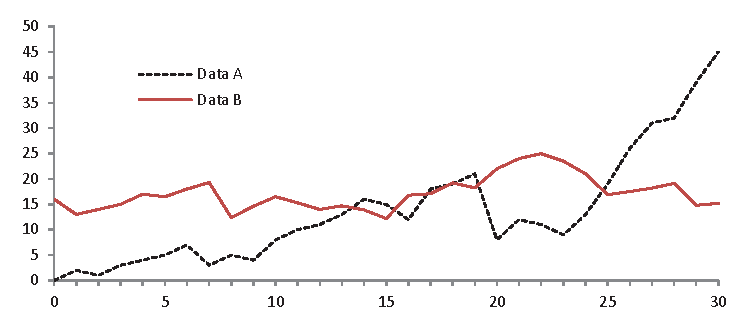
\includegraphics[width=\textwidth]{fig1.eps}
% \caption{A figure caption is always placed below the illustration.
% Please note that short captions are centered, while long ones are
% justified by the macro package automatically.} \label{fig1}
% \end{figure}
% 
% \begin{theorem}
% This is a sample theorem. The run-in heading is set in bold, while
% the following text appears in italics. Definitions, lemmas,
% propositions, and corollaries are styled the same way.
% \end{theorem}
% %
% % the environments 'definition', 'lemma', 'proposition', 'corollary',
% % 'remark', and 'example' are defined in the LLNCS documentclass as well.
% %
% \begin{proof}
% Proofs, examples, and remarks have the initial word in italics,
% while the following text appears in normal font.
% \end{proof}
% For citations of references, we prefer the use of square brackets
% and consecutive numbers. Citations using labels or the author/year
% convention are also acceptable. The following bibliography provides
% a sample reference list with entries for journal
% articles~\cite{ref_article1}, an LNCS chapter~\cite{ref_lncs1}, a
% book~\cite{ref_book1}, proceedings without editors~\cite{ref_proc1},
% and a homepage~\cite{ref_url1}. Multiple citations are grouped
% \cite{ref_article1,ref_lncs1,ref_book1},
% \cite{ref_article1,ref_book1,ref_proc1,ref_url1}.
%
% ---- Bibliography ----
%
% BibTeX users should specify bibliography style 'splncs04'.
% References will then be sorted and formatted in the correct style.
%
\bibliographystyle{splncs04}
\bibliography{main}
%
% \begin{thebibliography}{8}
% \bibitem{ref_article1}
% Author, F.: Article title. Journal \textbf{2}(5), 99--110 (2016)
% 
% \bibitem{ref_lncs1}
% Author, F., Author, S.: Title of a proceedings paper. In: Editor,
% F., Editor, S. (eds.) CONFERENCE 2016, LNCS, vol. 9999, pp. 1--13.
% Springer, Heidelberg (2016). \doi{10.10007/1234567890}
% 
% \bibitem{ref_book1}
% Author, F., Author, S., Author, T.: Book title. 2nd edn. Publisher,
% Location (1999)
% 
% \bibitem{ref_proc1}
% Author, A.-B.: Contribution title. In: 9th International Proceedings
% on Proceedings, pp. 1--2. Publisher, Location (2010)
% 
% \bibitem{ref_url1}
% LNCS Homepage, \url{http://www.springer.com/lncs}. Last accessed 4
% Oct 2017
% \end{thebibliography}

\blue{We solicit submissions in the form of regular research papers describing original scientific research results, including system development and case studies. Regular research papers should not exceed 18 pages in the Springer LNCS format, including bibliography and figures. This category encompasses both theoretical and implementation (also known as system descriptions) papers. In either case, submissions should clearly identify what has been accomplished and why it is significant. Submissions will be judged on the basis of significance, relevance, correctness, originality, and clarity. System descriptions papers should contain a link to a working system and will be judged on originality, usefulness, and design. In case of lack of space, proofs, experimental results, or any information supporting the technical results of the paper could be provided as an appendix or a link to a web page, but reviewers are not obliged to read them.}
\end{document}
